\documentclass[12pt]{article}

\usepackage[utf8]{inputenc}
\usepackage[T1]{fontenc}  
\usepackage[francais]{babel}   
\usepackage{fancyhdr}
\usepackage[top=2.5cm,bottom=2.5cm,left=2.5cm,right=2.5cm]{geometry}
\usepackage{lmodern}
\usepackage{listings}
\usepackage{color}
\usepackage{blindtext}
\usepackage[colorlinks=true,urlcolor=black,linkcolor=black]{hyperref}
\definecolor{grey}{rgb}{0.3,0.3,0.3}
\usepackage{graphicx}

\lstset{
language=C++,
basicstyle=\footnotesize\ttfamily,
numberstyle=\normalsize,
numbersep=7pt,
keywordstyle=\color{blue},
commentstyle=\color{grey}
}

\newcommand\Titre{TP4 : Héritage, Polymorphisme}
\newcommand\Dater{Pour le 6 février 2015}
\newcommand{\Numbi}{B3425}
\newcommand{\Membres}{\textsc{Bai} Emilien,
\newline \textsc{Haidara} Mohamed}

\title{\Titre \newline \large Document de conception}
\author{Bin\^ome \Numbi{}: \Membres}
\date{\Dater}

\begin{document}

\pagestyle{fancy}
\renewcommand{\footrulewidth}{1pt}
\renewcommand{\headheight}{1cm}
\renewcommand{\contentsname}{Table des matières}



\lhead{\Membres}
\chead{\Titre}
\rhead{\Numbi}

\begin{center}
\begin{LARGE}
\begin{bfseries}

\vspace{1\baselineskip}

\underline{\Titre}
~\newline~\newline \begin{large} Document de conception\end{large}
\end{bfseries}
\end{LARGE}
\end{center}

\tableofcontents

\section*{Introduction}
Dans ce 4ème TP de C++ il nous était demandé d'implémenter un éditeur de formes géométriques : \textit{ Cercle, Rectangle, Ligne, Polyligne } et certaines opérations sur ces formes telles que la suppression, le déplacement, la sélection.
Les objectifs du TP étaient principalement de (re)voir des notions telles que:
\begin{itemize}
\item l'héritage
\item le polymorphisme
\item l'utilisation des design pattern (ou patrons de conception)
\item l'évaluation des performances d'un programme
\end{itemize}
Nous avons ainsi pu mettre en pratique les notions vues en cours. Dans ce document vous trouverez une explication détaillée de notre programme et des choix effectués. 


\section{Conception}
\subsection{Design Pattern}
Pour la réalisation du TP, nous avons combiné deux design patterns :
\begin{itemize}
\item \textbf{Pattern Singleton :} qui permet de restreindre l'instanciation d’une classe à un seul objet. Ainsi il n’y aura qu’une seule instance de la classe principale qui sera accessible par les autres classes qui en auront besoin directement notamment les commandes.
\item \textbf{Pattern Commande :} qui permet une séparation optimale du code initiateur de l’action du code de l’action elle-même. A Chaque commande, doit correspondre une classe qui possède deux méthodes publiques : une permettant d’exécuter la commande, l’autre d’annuler l’effet de la commande. 
\end{itemize}
De l’utilisation de ces deux commandes, a découlé une séparation de l’application en deux grosses parties :
\begin{itemize}
\item le \textbf{c\oe{}ur} de l’application appelée \textbf{Modele} (cf. figure \ref{fig:Modele}) avec une seule instance (geoEdit) composée de classes représentant les différentes formes géométriques.
\item la classe \textbf{Commande} (cf. figure \ref{fig:Commande}) avec ses descendants permettant de gérer les entrées et sorties. Cette modélisation permet dans le futur de réutiliser le c\oe{}ur de l’application avec une interface graphique par exemple
\end{itemize}

\subsection{Diagramme de Classes}
Une version d'une meilleur résolution du diagramme de classe est fournie dans le répertoire ./doc. Il s'agit du fichier \textit{ B3425Diagramme.pdf}. 
\begin{figure}[!h]
\begin{center}
\includegraphics*[scale = 0.40]{Tp4Modele.png}
\caption{C\oe{}ur de l'application}
\label{fig:Modele}

\end{center}
\end{figure}

\begin{figure}
\begin{center}
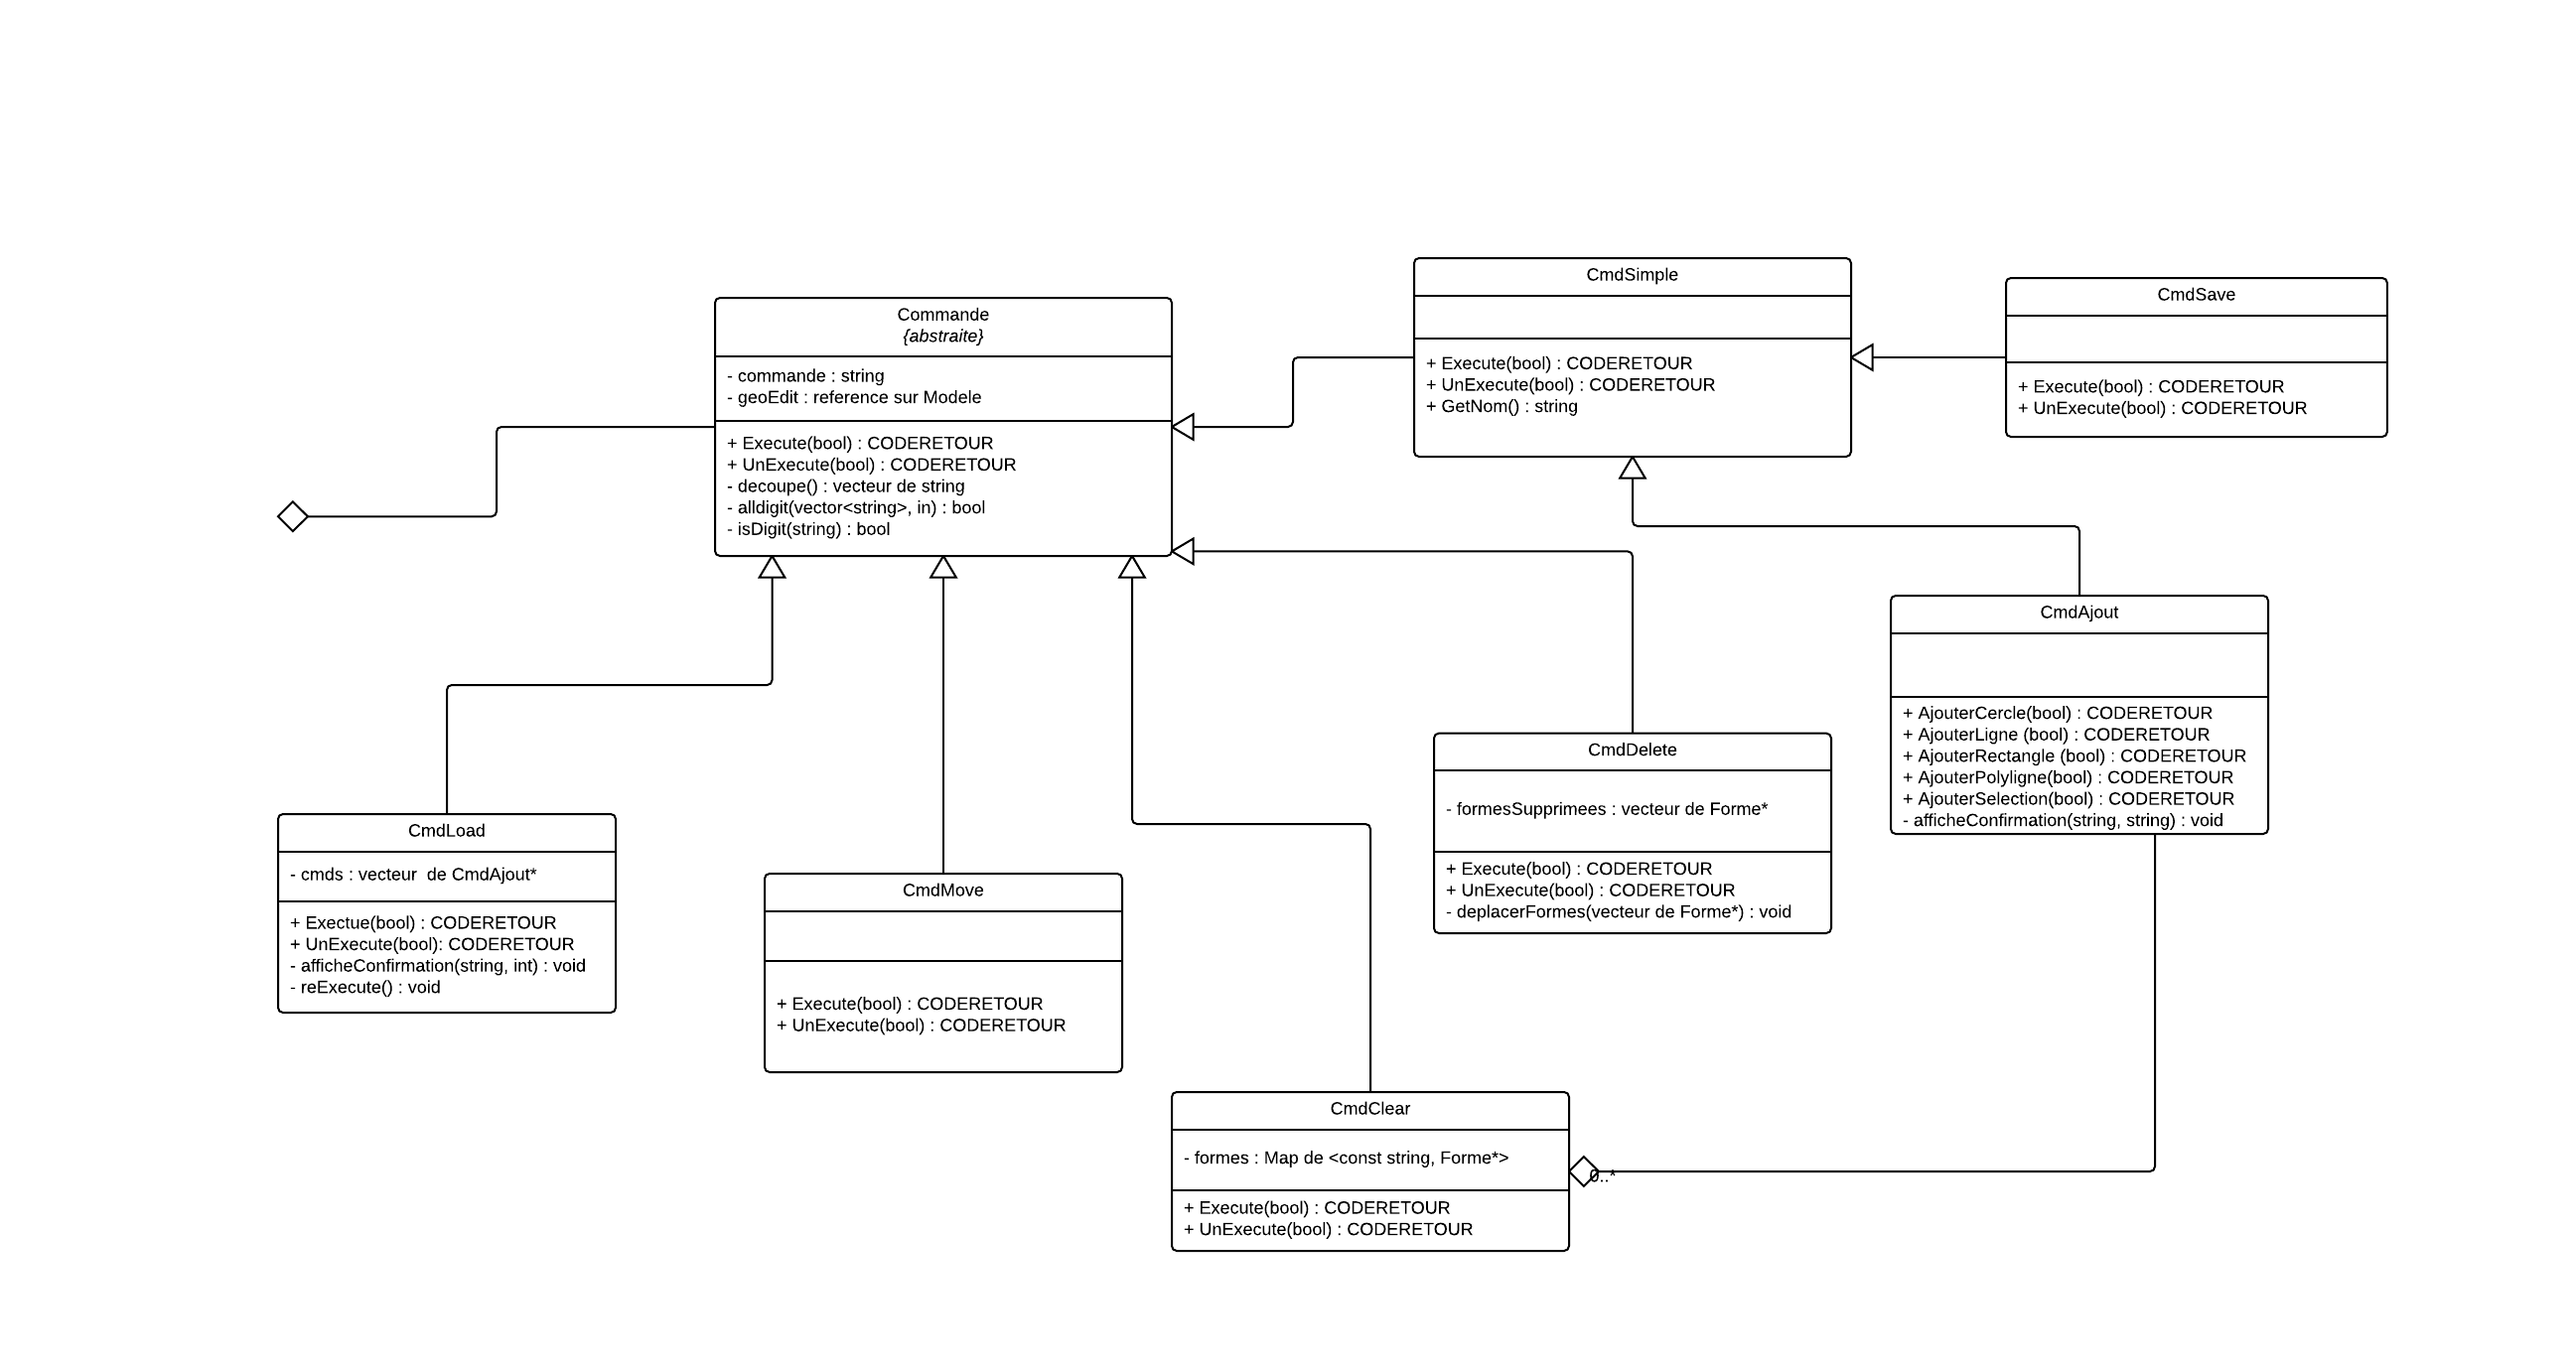
\includegraphics[scale = 0.44]{Tp4Commande.png}
\caption{Commande}
\label{fig:Commande}
\end{center}
\end{figure}

\section{Spécifications}
Ici seront présentées les principales classes et leur méthodes et l’interaction qui se fait entre les classes.
\subsection{Modele et Commande}
La classe Modele, en tant que classe principale, peut être vue comme \textit{ une base de données} qui se charge de stocker toutes les formes et les commandes et fournis un certain nombre \textit{ d’opérations ou méthodes } aux commandes qui interagiront avec elles. 

Les formes sont stockées dans une MAP de type : \textit{ map<const string, Forme*> }. Ainsi une forme peut être retrouvée grâce à son nom.
\\A coté de cela, nous avons deux piles de pointeurs sur Commande permettant de gérer le UNDO et le REDO des commandes exécutées : 
\newline
\begin{itemize}
\item \textbf{Undo :} Cette méthode de la classe principale vérifie si la pile \textit{ cmdToUndo} est vide. Si ce n'est pas le cas, annule la dernière commande ayant modifiée le modèle grâce à la méthode \textbf{UnExecute} de la classe commande, empile cett sur la pile \textit{cmdToRedo} et dépile \textit{cmdToUndo}.
\item \textbf{Redo :} Exécute les mêmes actions mais en dépilant	\textit{cmdToRedo} pour empiler sur \textit{cmdToUndo} et appelle la méthode \textbf{Execute}. \\
Les opérations d'empilement sont effectuées grâce à la méthode \textbf{void Empiler} qui videra la pile \textit{cmdToRedo} à chaque empilement. Il est à noter que toutes les commandes ne sont pas \textit{undoable} comme par exemple la commande LIST, SAVE et la commande de création d'une sélection. Notre architecture gère un nombre indéterminé de UNDO et REDO contrairement à la limite de 20 qui avait été fixée.
\end{itemize}

Tous les objets de la classe Commande partagent un \textbf{attribut static geoEdit} qui référence la classe principale Modele. Ainsi chaque objet Commande pourra modifier directement le Modele et ils partageront tous le même état de \textit{ la base de données.} Parmi les principales, méthodes fournies par le Modele, on peut citer :
\newline
\begin{itemize}
\item \textbf{void Ajouter(string name, Forme * forme ) :}

Cette méthode reçoit une Forme crée par une Commande et l’ajoute dans la map. Les vérifications sont effectuées par la commande qui s’assure qu’une autre forme ayant le même nom ne soit pas déjà présente à travers une méthode fournie par la classe principale.

\item \textbf{void Clear() :}

Supprime toutes les formes actuellement présentes dans la map. Mais avant de supprimer les formes, on réalise une copie au préalable. Ce mécanisme permet d’optimiser l’annulation de la commande CLEAR qui n’aura pas à récréer toutes les formes qui étaient déjà présentes dans la map.
\end{itemize}
Une autre optimisation a été au niveau de la commande LOAD plus précisément la classe \textit{ cmdLoad} qui permet de charger un ensemble de Forme à partir d'un fichier. Cette classe est composée d'autres commandes appelées \textit{cmdAjout} qui se chargeront de vérifier la syntaxe de toutes les lignes du fichier. Après avoir lu un fichier, on garde une indépendance totale vis à vis de celui-ci ce qui permet de pouvoir UNDO et REDO un LOAD sans lire encore une fois le fichier.

\subsection{Forme}
Cette \textbf{classe abstraite} constitue la classe de base dont va hériter toutes les formes géométrique. Elle engendre directement les classe \textbf{Cercle}, \textbf{Polyligne} et \textbf{Selection}. La classe sélection est considérée comme une forme car cela rend plus facile la recherche lors d'un l'appel pouvant concerner une "vraie" forme ou une sélection (MOVE, DELETE\ldots)  Les classes \textbf{Ligne} et \textbf{Rectangle} héritent elles de Polyligne. Toutes ces classes ont en commun les méthodes
\begin{itemize}
\item\textbf{void Afficher (ostream \&)}\\
Cette méthode redéfinie l'affichage sur la sortie standard pour chacun des types de forme. Elle ne renvoie rien pour une sélection qui ne doit pas apparaître lors de l'affichage des formes. Elle permet aussi de sauvegarder les Forme dans un fichier en recevant le flux vers celui-ci.
\item \textbf{bool InclusDans(const \& Point, const \& Point)}\\
 Cette méthode permet de définir si la forme est contenue entièrement dans le rectangle formé par les deux points passés en paramètre. Comme il n'est pas possible de sélectionner une sélection, la méthode renvoie systématiquement \textbf{false}.
\item\textbf{void Deplacer (long, long)}\\
Cette méthode déplace point par point, la forme pour laquelle elle est appelée, ou dans le cas d'une sélection, appelle la méthode Deplacer pour chacune des formes la constituant.
\end{itemize}

\section{Tests}
\subsection{Présentation}
L’application que nous avons réalisé a subi une batterie de Test décomposée en deux catégories :
\begin{itemize}
\item Les tests des fonctions “de base” sans conflit possible ou erreur de syntaxe : ces tests modélisent une utilisation sans erreur de l’application. Ils reprennent les fonctions telles qu’ajouter des formes ou des sélections, les déplacer, les supprimer, ou encore tester l’annulation d’une commande, sa reprise, l’enregistrement de la figure courante ainsi que le chargement d’une figure existante.
\item Les tests des fonctions “avancées” de l’application : ces tests sont là pour vérifier que le programme ne plante pas en cas d’une utilisation différente de la syntaxe définie par le cahier des charges. Ce sont aussi des tests plus avancés cherchant à vérifier le bon déroulement de l'exécution de l'application même quand un enchaînement de commande est plus compliqué ou piégeux.
\end{itemize}
Pour la mémoire, on a utilisé \textit{valgrind} pour détecter les fuites de mémoire et l'utilisation de variables non initialisées.

\begin{figure}[!h]
\begin{center}
\begin{tabular}{|c|c|}
\hline
\textbf{\large{n\degres du test}} & \textbf{\large {Description du test}}\\
\hline
\multicolumn{2}{|c|}{\textbf{\large{Test des fonctions "de base"}}}\\
\hline
01 & Ajout Multiple et Lister\\
\hline
02 & Ajout d'un objet puis suppression\\
\hline
03 & Déplacement d'objet\\
\hline
04 & Déplacement d'une sélection\\
\hline
05 & Ajout de Forme puis UNDO\\
\hline
06 & Ajout de Forme puis UNDO puis REDO\\
\hline
07 & Suppression d'une sélection\\
\hline
08 & SAVE un fichier\\
\hline
09 & Test de la commande LOAD pour un fichier existant\\
\hline
10 & Test de la comande CLEAR\\
\hline
11 & Commande CLEAR puis UNDO\\
\hline
12 & Commande LOAD puis UNDO\\
\hline
13 & LOAD dans une application sans conflit de nom\\
\hline
14 & Enchainement LOAD UNDO REDO\\
\hline

\multicolumn{2}{|c|}{\textbf{\large{Test des fonctions "avancées"}}}\\
\hline
15 & Ajout de deux Formes ayant le même nom (conflit de nom)\\
\hline
16 & LOAD dans une application avec conflit de nom\\
\hline
17 & MOVE un objet inexistant\\
\hline
18 & MOVE un objet supprimé\\
\hline
19 & DELETE un objet inexistant\\
\hline
20 & DELETE un objet supprime\\
\hline
21 & DELETE selection, UNDO, MOVE sélection\\
\hline
22 & DELETE une forme d'une sélection puis UNDO puis MOVE la sélection\\
\hline
23 & Appel de UNDO plus de fois qu'il n'y a d'événement\\
\hline
24 & Appel de REDO plus de fois qu'il n'y a eu de UNDO\\
\hline
25 & Ajout avec mauvais parametres puis UNDO\\
\hline
26 & LOAD d'un fichier corrompu\\
\hline
27 & Ajout d'une forme ayant le nom d'une forme supprimee puis UNDOx2\\
\hline
28 & LOAD d'un fichier contenant des selections et test sur ces selections\\
\hline
29 & Enchainement de commandes non définies par le cahier des charges\\
\hline
\end{tabular}
\end{center}
\caption{Liste des Tests}
\label{tab:Liste des Tests}
\end{figure}
\subsection{Exécution}
Pour effectuer notre panel de test, nous avons réutilisé un script shell fourni lors d'un précédant TP. Ce script se trouve dans le répertoire ./tests et se nomme mktest.sh. Il exécute à la suite tous les textes définis dans la figure \ref{tab:Liste des Tests} et affiche sur la sortie standard le résultat unitaire de chaque test ainsi qu'un bilan répertoriant le nombre de tests passés, échoués ou mal formés. Lors de cette exécution, tous les tests que nous avons définis se sont exécutés avec succès. 

\section{Performances}
Nous avons aussi testé les performances de notre programme grâce à un script permettant à la fois de générer un fichier de commande qui sera passé en entrée de notre application. Nous appelons ensuite notre application plusieurs fois pour réaliser la moyenne des temps d'ajout nécessaires. Les tests ont été réalisés sur des machines du département, en enlevant les traces de la sortie standard (OK \ldots) qui ont étés pensées en compilation conditionnelle. Le document perfs\_B3425.pdf situé dans le répertoire doc/ consigne les résultats des tests effectués.

\end{document}